%---------change this every homework
\def\yourid{mst3k}
\def\collabs{list your collaborators}
\def\sources{Cormen, et al, Introduction to Algorithms; Adams, Douglas, Hitchhiker's Guide to the Galaxy}
% -----------------------------------------------------
\def\duedate{September 11, 2024 at 11:59p}
\def\pnumber{1}
%-------------------------------------

\documentclass[10pt]{article}
\usepackage{dsa2}
\usepackage{tikz-cd}
\usepackage{wrapfig}


\begin{document}
\thispagestyle{empty}
\handout

%----Begin your modifications here

%%%%%%%%%%%%%%%%%%%%%%%%%%%%%%%%%%%%%%%%%%%%%%%%%%%%%%%%
\begin{problem} Asymptotics \end{problem}
\begin{enumerate}
\item Consider the following functions, $f(n)=n^{1.5}$ and $g(n)=n (\log n)^2$. Which grows more quickly?  (That is, which would be a ``worse'' time-complexity.)  Express your answer in terms of one of the order-classes we've studied. If you can use little-omega $\omega$ or little-oh $o$, use that. If not, use big-Oh $O$ or big-Omega $\Omega$. Your answer will be of the form $f(n) = \Theta(g(n))$ but with something other than Big-Theta $\Theta$.  Explain your answer with a short proof; you may use any definitions from the course slides.
\end{enumerate}

\solution{
% Your solution here
}


%%%%%%%%%%%%%%%%%%%%%%%%%%%%%%%%%%%%%%%%%%%%%%%%%%%%%%%%
\begin{problem} Trick or Treat: Maximum Candy \end{problem}

October 31st is just around the corner and Prof. Bloomfield's children are making big plans for trick-or-treating in their neighborhood. In an attempt to limit the amount of candy his children can collect, Prof. Bloomfield -- being a mean father -- told them that they can only go 2 blocks away in any direction.  The children will be starting at their house, which happens to be next to an intersection, meaning that can choose one of 4 street segments to start on.  Each street segment has a number of houses that provide candy on it.  Given a map of the neighborhood, what will Prof. Bloomfield's dental bill be?


%\clearpage

\begin{wrapfigure}{r}{0.5\textwidth}
  \begin{center}
    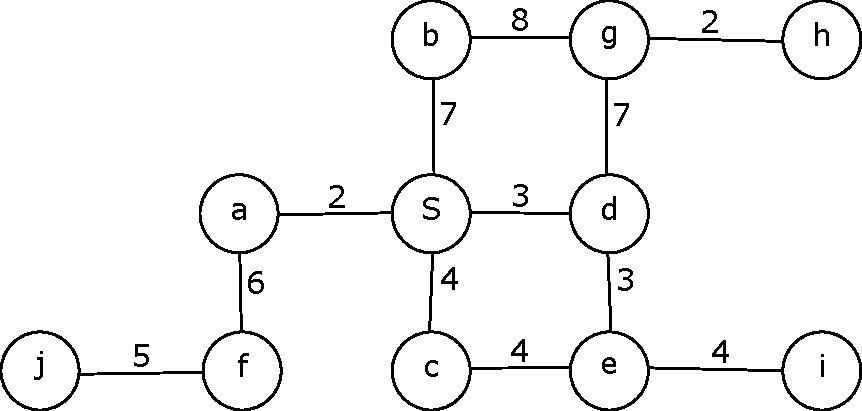
\includegraphics[width=0.48\textwidth]{halloween-graph.pdf}
  \end{center}
  \caption{Neighborhood roads}
\end{wrapfigure}

Rather, how much candy can each child collect?

The map can be visualized as a graph containing nodes (intersections) and edges (street segments). Edge weights represent the number of houses that provide candy on a given street segment.  In the figure to the right, if the children start at node S (in the middle of the graph), there are three streets (edges) that they cannot travel to, as they are more than 2 blocks away: J-F, G-H, and E-I.  The total candy they can collect is the sum of the other edges, or 44.

Given a weighted, connected, unidirectional graph $G=(V,E)$, a designated start vertex $s$, and a parameter $n$ (the maximum number of blocks that can be traveled), create an algorithm that finds the amount of candy that the children can collect. Clearly describe your algorithm. Analyze and state the time complexity of your algorithm using asymptotic notation.   {\em Note that your algorithm must work for {\bf any} graph, not just the one shown here.}
\vskip 2em



\solution{
% Your solution here
}

%%%%%%%%%%%%%%%%%%%%%%%%%%%%%%%%%%%%%%%%%%%%%%%%%%%%%%%%
\begin{problem} Trick or Treat: Parental Supervision \end{problem}

Given the number of children that will be trick-or-treating in Prof. Bloomfield's neighborhood, he really thinks parents should be watching the streets. When a parent is present at a given intersection they can see each street segment that connects to that intersection.

Use the same graph representation as in the previous problem. Note that while the graph above is orthogonal (all the streets are on a grid, the provided graph may not be -- there may be any number of roads connecting to an intersection, a block of three streets (edges), etc. Create an algorithm that finds the minimal number of parents needed such that each street segment has a parent stationed at one of the connecting intersections. In the graph above, the answer is 4 (nodes E, F, G, and S).  Clearly describe your algorithm. Analyze and state the time complexity of your algorithm using asymptotic notation.  {\em Note that your algorithm must work for {\bf any} graph, not just the one shown above.} 
\vskip 2em


\solution{
% Your solution here
}


\end{document}
